\section{Results}

\subsection{Hyperparameter Search and Model Fitting}

Throughout this section we use the \textit{stm} package, which is implemented in the R programming language (\citealp{stm}). The most important hyperparameter choice when fitting an STM is the number of topics, $K$. While there is no \textit{true} or \textit{optimal} number of topics, we explore the hyperparameter space using the \textit{searchK} function to get an understanding of the impact of $K$ on model fit. We use four of the metrics that come with this function, \textit{held-out likelihood}, \textit{semantic coherence}, \textit{exclusivity}, and \textit{residuals}.

The \textit{held-out likelihood} approach is based on document completion. The \textit{searchK} function randomly holds out a proportion of some of the documents; both the number of documents from which a portion is held out and the respective held-out proportions can be specified by the user. This gives rise to a set of held-out words for which the likelihood is calculated, given the trained model. Thus, the higher this held-out likelihood, the more predictive power the model has on average. For more detailed information on held-out likelihood based on document completion and other types of held-out likelihoods, see \cite{wallach2009evaluation}.

Regarding the second metric, first introduced by \cite{mimno2011optimizing}, a model with $K$ topics is \textit{semantically coherent} whenever those words that characterize a specific topic $k$ (i.e., the most frequent words within topic $k$) also do appear in the same documents. In order to formally define semantic coherence, let first $D(v)$ be the \textit{document frequency} of word $v$ (that is, the number of documents where $v$ occurs at least once) and let $D(v, v')$ be the \textit{co-document frequency} of words $v$ and $v'$ (that is, the number of documents where both $v$ \textit{and} $v'$ occur at least once). Furthermore, consider the $M$ most probable words in a given topic $k$. Then, semantic coherence for topic $k$, $C_{k}$, is defined as follows:
\begin{align*}
C_{k} &= \sum_{i=2}^{M}\sum_{j=2}^{i-1}\log(\frac{D(v_{i}, v_{j})+1}{D(v_{j})}).
\end{align*}
That is, semantic coherence is the sum of (logarithmized) proportions of word co-occurrences to total word occurrences, the additive factor $1$ in the numerator simply being a smoothness adjustment. It becomes apparent that by having some words that are very frequent across a couple of documents, we could achieve high semantic coherence without our topics being semantically coherent at all once we look beyond these common words (\citealp{stm, mimno2011optimizing}). As a partial remedy, we previously excluded some of such overly frequent words (see section 3.2).

A natural "counter-metric" of semantic coherence is \textit{exclusivity}, which basically tells us to which degree words within a given topic \textit{only} occur in that topic. To formalize this, first define the empirical frequency of word $v$, $v\in{V}$, within topic $k$ as $\hat{\beta}_{k,v}$.\footnote{We use $\hat{\beta}_{k,v}$ for empirical frequencies (i.e., word counts) within topic $k$ to distinguish them from the (normalized) word probabilities $\beta_{k,v}$.} These empirical frequencies are then normalized across all topics $k\in\{1,...,K\}$. This way, the normalized frequencies now represent the probability of observing topic $k$, conditional upon the word being $v$ - that is, the exclusivity of word $v$ regarding topic $k$. Formally, exclusivity of word $v$ to topic $k$, $E_{k,v}$, is thus defined as:
\begin{align*}
E_{k,v} &= \hat{\beta}_{k,v}/\sum_{j=1}^{K}\hat{\beta}_{j,v}.
\end{align*}
Combining a word's frequency and exclusivity finally yields its Frequency-Exclusivity (\textit{FREX}) score, explained in more detail in section 4.2 below and in \cite{bischof2012summarizing}.

Finally, \textit{residuals} is a metric based on residual dispersion. Recall that $z_{d,n}$ is drawn from a $K$-category multinomial distribution, which is a member of the exponential family. Therefore, its dispersion parameter is equal to one, according to theory. This way, an observed residual dispersion larger than one roughly indicates that the number of topics $K$ was most likely chosen insufficiently small. See \cite{taddy2012estimation} for a detailed derivation.

Another aspect to be taken into account when choosing $K$ (or, to be precise, when choosing a search grid for searchK) is interpretability. While a large $K$ certainly allows for a more fine-grained determination of topics, the resulting topics might be rather difficult to label. Furthermore, for large $K$ we would obtain many topics which could be considered sub-topics of the topics we would obtain when using a smaller value for $K$. As a consequence, we select a search grid between 5 and 40, in steps of 5. Before fitting the model, we need to choose the document-level covariates we want to include. Since a topic model is explorative by definition, we simply include those covariates that seem to be most influential \textit{a priori}: party and state (both categorical), date (as smooth effect), as well as percentage of immigrants, GDP per capita, unemployment rate, and the 2017 election results of the MP's respective party (the last four as smooth effects and on an electoral-district level). We choose degrees of freedom (\textit{df}) = 5 for all smooth effects to avoid spurious wiggles due to overfitting.\footnote{The graphical illustrations of the relationship between topic proportions and continuous covariates in sections 4.4 through 4.7 suggest that df = 5 is indeed sufficient.} No topical content variable is included at this stage.

The graph below shows the four metrics, as introduced above, for values of $K$ between 5 and 40 (in steps of 5). Both 15 and 20 topics seem to be good trade-offs between the metrics used. As mentioned above, no true or optimal $K$ exists. Taking into account the interpretability aspect, we opt for $K$ = 15. For comparison, we also conducted the subsequent analysis for $K$ = 6 and $K$ = 20. In general, the topics generated are similar, but for $K$ = 6 only around three of them are clear-cut, while for $K$ = 20 some topics could easily be grouped together. This further corroborates our choice that $K$ = 15 indeed seems to be a good trade-off. Our model thus uses $K$ = 15 as hyperparameter. For model fitting, we again need to choose document-level covariates. We initially select the same model specifications as in the hyperparameter search above (see sections 4.5 and 4.6 for modifications).

\begin{figure}[h!]
  \centering
  \captionsetup{justification=centering,margin=2cm}
  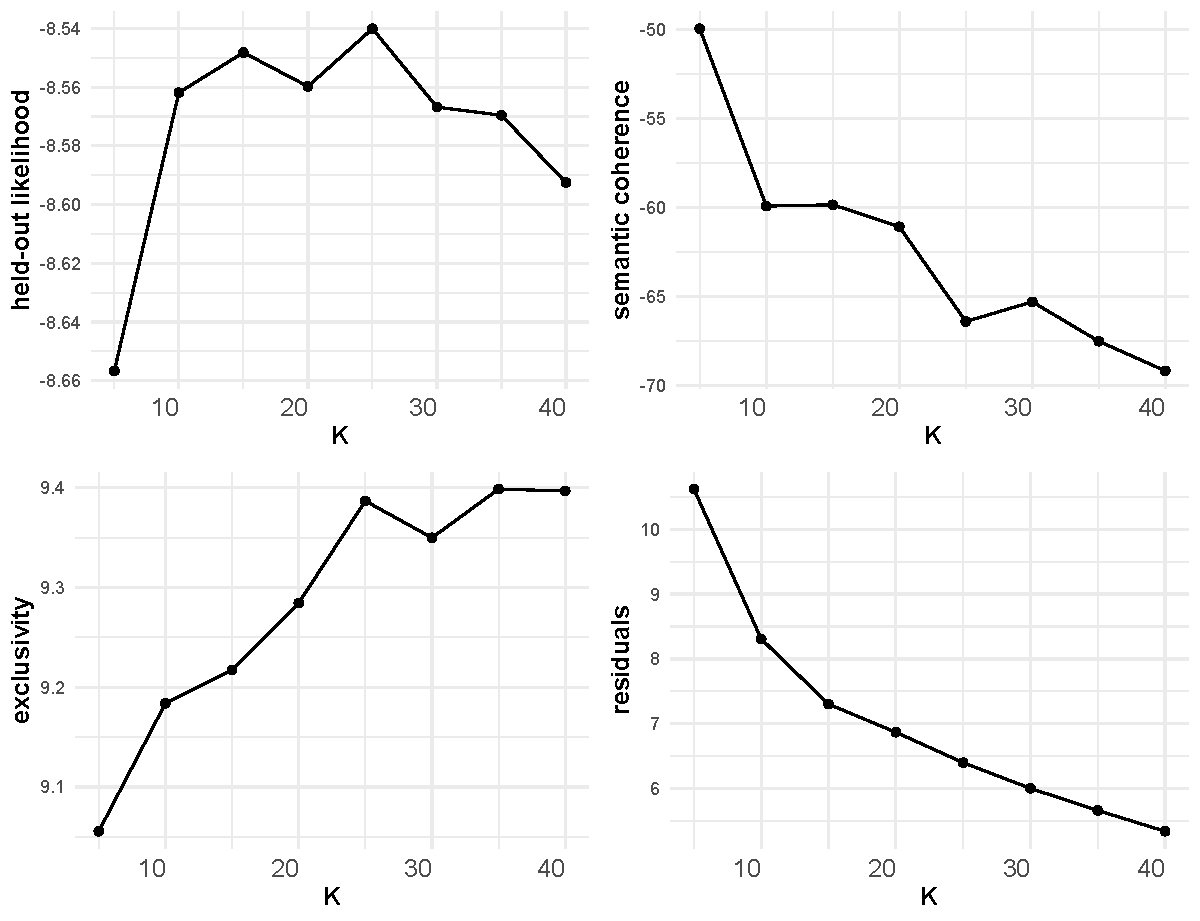
\includegraphics[scale = 0.5]{../plots/4_1/searchK.pdf}
  \caption{Model evaluation metrics for hyperparameter K (number of topics).}
  \label{fig:searchK}
\end{figure}

\subsection{Labeling}

As a first step after fitting the model, we would like to visually inspect the resulting topics, in particular their most representative words. However, representativeness of words for a given topic depends on the weighting metric used. The STM comes with four topic-word metrics - \textit{highest probability}, \textit{FREX}, \textit{Lift}, and \textit{Score} - which are discussed in the following.

Given a topic $k$, \textit{highest probability} simply outputs those words in the topic-specific empirical word vector $\hat{\beta}_{k}$ with the highest corpus frequency, i.e, those with the highest absolute frequency across all documents within topic $k$. Using the same notation as in section 4.1 above, let $\hat{\beta}_{k,v}$ again be the empirical frequency of word $v$ within topic $k$. Then the highest probability word within topic $k$ is simply $\underset{v \in V}{\operatorname{argmax}\hat{\beta}_{k,v}}$. This relatively simple measure only takes into account how often words occur in absolute terms, but not how specific those words are to the given topic. This is why we observe words like \textit{wichtig}, \textit{berlin}, or \textit{frag} within the highest probability words for several topics. And since such words are very common, unspecific words, they are not particularly useful for distinguishing or labeling topics.

To also account for the degree to which a word \textit{exclusively} belongs to a certain topic, we also consider the top words according to the \textit{FREX} metric. It takes into account not only how frequent but also how exclusive words are. Formally, the FREX score of word $v$ with respect to topic $k$ is calculated as follows:
\begin{align*}
FREX_{k,v} &= (\frac{\omega}{ECDF(\hat{\beta}_{k,v}/\sum_{j=1}^{K}\hat{\beta}_{j,v})} + \frac{1-\omega}{ECDF(\hat{\beta}_{k,v})})^{-1} &= (\frac{\omega}{ECDF(E_{k,v})} + \frac{1-\omega}{ECDF(\hat{\beta}_{k,v})})^{-1},
\end{align*}
where $\omega$ is the weight  assigned to exclusivity (set to 0.7 by default in the STM), $E_{k,v}$ is the word's exclusivity as defined in section 4.1, and \textit{ECDF} is the empirical CDF. Thus, for a given topic, $FREX_{k,v}$ is simply the harmonic mean of i) the rank of word $v$ by frequency within topic $k$ (frequency rank) and ii) the rank of topic $k$ by the frequency of word $v$, across all topics $j \in \{1,...,K\}$ (exclusivity rank). Further information on the estimation of \textit{FREX} can be found in \cite{stm} and in \cite{bischof2012summarizing}.

\textit{Lift} is another topic-word metric, where the frequency of word $v$ within topic $k$,  $\hat{\beta}_{k,v}$, is weighted by the inverse of $v$'s relative frequency across the entire corpus, i.e., $v$'s empirical corpus probability. Formally:
\begin{align*}
Lift_{k,v} &= \hat{\beta}_{k,v}/(\omega_{v}/\sum_{v}\omega_{v}),
\end{align*}
where $\omega_{v}$ denotes the word count of word $v$ in the entire corpus. This way, Lift gives larger weight to those words that rarely appear in other topics. Further information on Lift can be found in \cite{taddy2012estimation}.

Finally, the \textit{Score} metric for word $v$ and topic $k$ is formally defined as:
\begin{align*}
Score_{k,v} &= \hat{\beta}_{k,v}(\log\hat{\beta}_{k,v} - 1/K\sum_{j}^{K}\log\hat{\beta}_{j,v}).
\end{align*}
Thus, Score weights word $v$'s frequency within topic $k$, $\beta_{k,v}$, by the difference between $v$'s log frequency within topic $k$ and the average of $v$'s log frequencies across all $K$ topics. This can roughly be interpreted as: $\beta_{k,v}$ is weighted by the proportion of $v$'s log frequency within topic $k$ to $v$'s average logarithmic frequency across all topics. For further information on the Score metric, see the R package \textit{lda} (\cite{chang2010package}).

To get a broad overview of which words characterize each one of the topics, the output below shows the five top words according to each of the four topic-word evaluation metrics, for three selected topics (see appendix XXX for top words of all topics).

\vspace{0.5cm}
\noindent
\textit{Topic 1 Top Words:}\\
 	 \textbf{Highest Prob:} buerg, link, merkel, frau, sich \\
 	 \textbf{FREX:} altpartei, islam, linksextremist, asylbewerb, linksextrem \\
 	 \textbf{Lift:} eitan, 22jaehrig, abdelsamad, abgehalftert, afdforder \\
 	 \textbf{Score:} altpartei, linksextremist, frauenkongress, islamist, boehring \\
\textit{Topic 3 Top Words:}\\
 	 \textbf{Highest Prob:} brauch, wichtig, leid, dank, klar \\
 	 \textbf{FREX:} emissionshandel, soli, marktwirtschaft, feedback, co2steu \\
 	 \textbf{Lift:} aequivalenz, altersvorsorgeprodukt, bildungsqualitaet, co2limit, co2meng \\
 	 \textbf{Score:} emissionshandel, co2limit, basisrent, euet, technologieoff \\
\textit{Topic 6 Top Words:}\\
 	 \textbf{Highest Prob:} gruen, klimaschutz, brauch, klar, euro \\
 	 \textbf{FREX:} fossil, erneuerbar, kohleausstieg, verkehrsminist, verkehrsw \\
 	 \textbf{Lift:} abgasbetrug, abgebaggert, abschalteinricht, abschaltet, ammoniak \\ 
 	 \textbf{Score:} erneuerbar, fossil, zdebel, verkehrsminist, klimaschutz \\

\noindent
A key task of topic analysis is to actually ascribe a meaning to the topics identified, i.e., to label them. While this is clearly where human judgment should and does come into play, we attempt to conduct the labeling in a more strategic (and thus less subjective) manner, following a 3-step procedure. This procedure is exemplified by topic 1. First, we consider the \textit{words} contained in the topic, for instance by simply inspecting the top words (see output above). For a better visualization, we use a word cloud. As shown below, for a given topic (i.e., conditional upon a specific topic being chosen), it shows highest probability words weighted by their frequency. Judging at first sight, topic 1 appears to be about right-wing nationalist issues, particularly immigration.

\begin{figure}[h!]
  \centering
  \captionsetup{justification=centering,margin=2cm}
  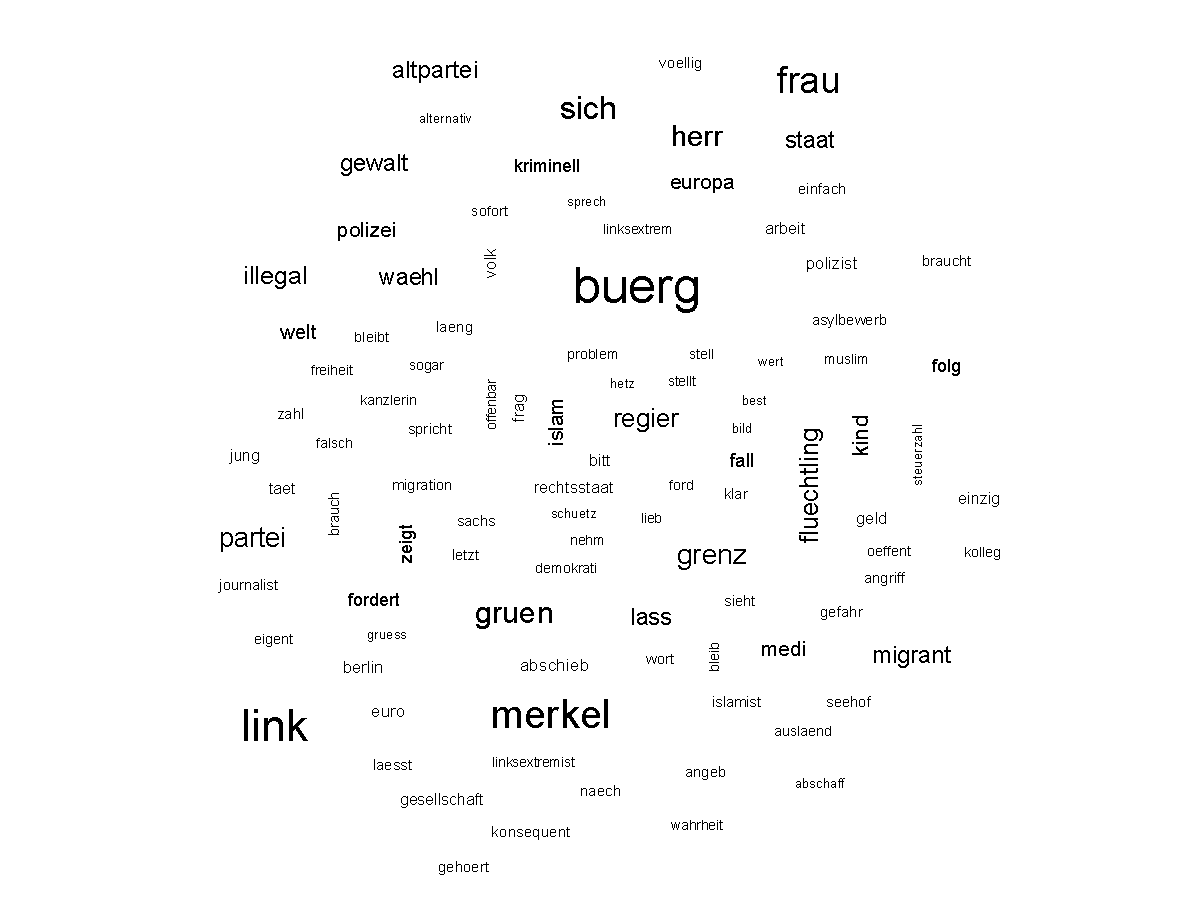
\includegraphics[scale = 0.5]{../plots/4_2/t1_wordcloud.pdf}
  \caption{Word cloud for topic 1.}
  \label{fig:t1_wordcloud}
\end{figure}

Second, to get a more thorough insight into the topic, we take a look at those documents that show the highest proportion for topic 1; that is, we consider the corresponding original, unprocessed tweets. The most representative document for topic 1 has a topic proportion $\theta_1$ equal to 98.86\%. It contains tweets from MP Martin Hess, a member of the AfD party from Baden-Württemberg, during June 2018. That is, MP Martin Hess tweeted almost exclusively about topic 1 during June 2018. The monthly document starts with:

\vspace{0.5cm}
\noindent
\textit{"Ehem. Verfassungsrichter bestätigt AfD-Forderung: Zurückweisung illegaler Migranten dringend geboten. Gegenwärtige Politik widerspricht dem Verstand und auch der Verfassung. Wir müssen zurück zu Recht \& Ordnung, wie die \#AfD seit fast 3 Jahren fordert!"}
\vspace{0.5cm}

The second most representative document for topic 1, with an almost identical $\theta_1$ = 98.37\%, is from the same MP, this time from May 2018. The document begins with:

\vspace{0.5cm}
\noindent
\textit{"Mio-Überweisungen u.a. an Kanzleien unter \#BAMF-Außenstellenleiterin, die mit Anwälten bandenmäßig Asylbetrug begangen haben soll. Und die Frau ist noch frei und präsentiert sich als Gutmensch. \#Staatsanwaltschaft muss hier handeln und Haftgründe prüfen."}
\vspace{0.5cm}

The documents exclusively focus on immigration issues, confirming the first impression gained through top words and word cloud: topic 1 concerns right-wing nationalist issues, in particular immigration. As a third step in our labeling process we finally assign a label to the topic: in this case, "Right/Nationalist". We repeat this 3-step procedure (inspecting top words and word cloud, reading through top documents, assigning a 1- or 2-word label) for all remaining topics, arriving at the following manual labels:

\begin{table}[h!]
	\centering
	\captionsetup{justification=centering,margin=2cm}
	\begin{tabular}{|l|l|}
	\hline
	Topic1  & Right/Nationalist    \\ \hline
	Topic2  & Miscellaneous 1      \\ \hline
	Topic3  & Climate Economics    \\ \hline
	Topic4  & Social/Housing       \\ \hline
	Topic5  & Digital/Future       \\ \hline
	Topic6  & Climate Protection   \\ \hline
	Topic7  & Europe               \\ \hline
	Topic8  & Corona               \\ \hline
	Topic9  & Left/Anti-war        \\ \hline
	Topic10 & Twitter/Politics 1   \\ \hline
	Topic11 & Twitter/Politics 2   \\ \hline
	Topic12 & Miscellaneous 2      \\ \hline
	Topic13 & Twitter/Politics 3   \\ \hline
	Topic14 & Right-wing Extremism \\ \hline
	Topic15 & Society/Solidarity   \\ \hline
	\end{tabular}
	\caption{List of topic labels.}
	\label{Tab:labels}
\end{table}

\subsection{Global-level Topic Analysis}

Next, we identify two ways to calculate global topic proportions (for a given topic $k$): either as simple (unweighted) average of $\theta_{d,k}$ across all documents (i.e., as the average of MP-level proportions across all MPs): $\frac{1}{D}\sum_{d=1}^{D}\theta_{d,k}$; or by first weighting each $\theta_{d,k}$ by the number of words in the respective documents, $N_d$, and then averaging across documents. The table below shows all topics with their respective global proportions for both weighting methodologies. We observe that for most topics, weighted and unweighted proportions are rather similar, but there are exceptions. In particular, the topics concerned with everyday political tweets have much higher unweighted than weighted frequencies; this makes sense, however, since such "diplomatic" tweets tend to be shorter than those discussing specific content.

\begin{figure}[h!]
  \centering
  \captionsetup{justification=centering,margin=2cm}
  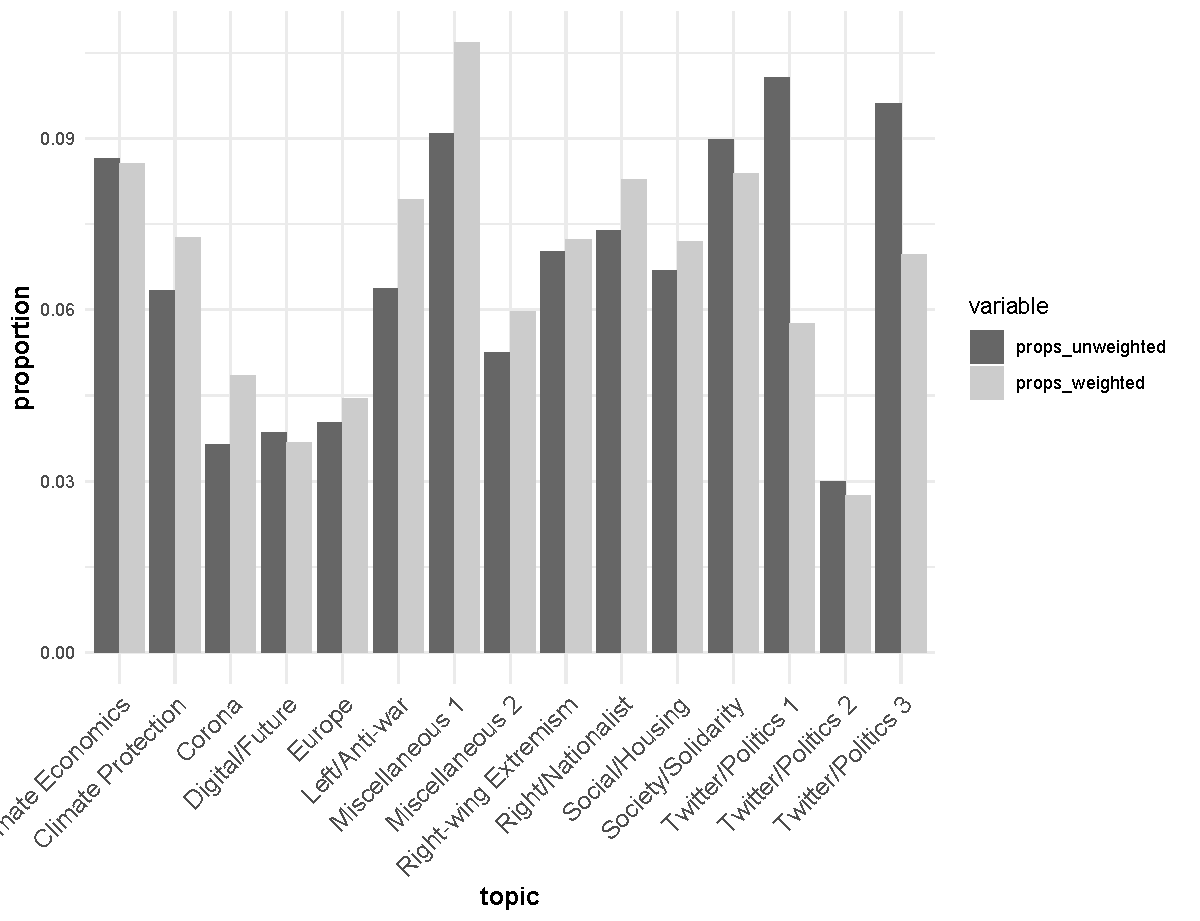
\includegraphics[scale = 0.5]{../plots/4_3/global_thetas.pdf}
  \caption{Weighted and unweighted global topic proportions.}
  \label{fig:global_thetas}
\end{figure}

While labeling tells us which words best represent each topic - and thus, what each topic truly represents - it does not yet tell us to which extent individual topics are related to each other. In the graph below, we visualize the similarity of two topics, Topic 3 (Climate Economics) and Topic 6 (Climate Protection), in terms of their vocabulary usage. As suggested by the topic labels already, there is a significant overlap in vocabulary usage.

\begin{figure}[h!]
  \centering
  \captionsetup{justification=centering,margin=2cm}
  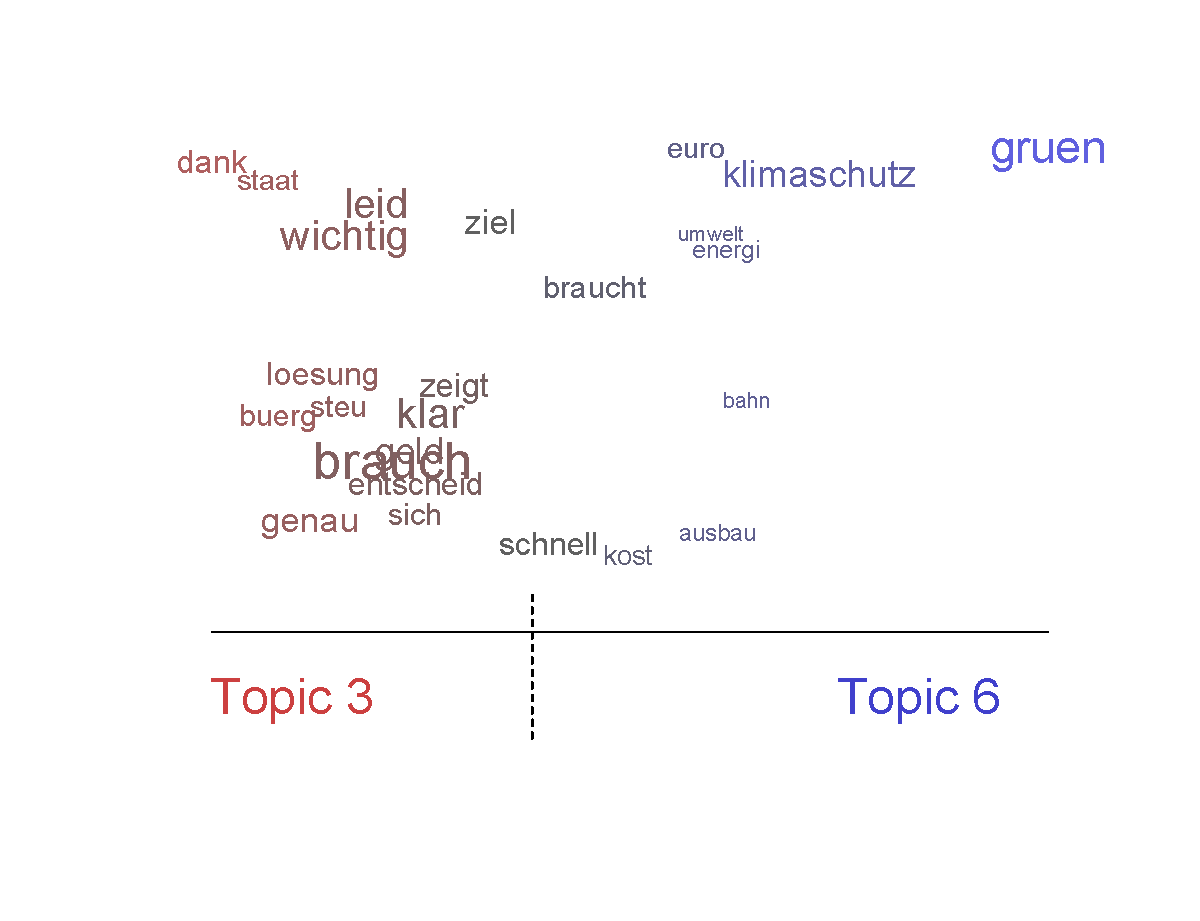
\includegraphics[scale = 0.5]{../plots/4_3/vocabulary_comparison.pdf}
  \caption{Comparison of vocabulary usage for two topics.}
  \label{fig:vocabulary_comparison}
\end{figure}

More generally, we can evaluate the connectedness between different topics by means of a matrix of correlations between document-level topic proportions $\theta_d$. This is visualized in Figure \ref{fig:topic_correlations} (left panel). Most topics are negatively correlated with each other, which does not come as a surprise given the relatively low total number of topics, 15, and that topic proportions are “supplements”: the higher one topic proportion, the lower the total of the others. Moreover, most topic correlations are rather weak in absolute size: the strongest negative correlation (-19.84\%) is the one between topic 1 (Right/Nationalist) and topic 15 (Society/Solidarity), while the strongest positive correlation (11.79\%) occurs between topic 10 (Twitter/Politics 1) and topic 13 (Twitter/Politics 3). We can also visualize these correlations using a network graph (Figure \ref{fig:topic_correlations}, right panel), where topics are connected by a dashed line whenever they are positively correlated. We observe three small clusters as well as some isolated topics, one of them being topic 8, Corona, which makes sense since this topic only entered the public sphere in early 2020, i.e., during the last months of our data collection period. In general, the relationships between the topics, as depicted below, are in line with their labeling.

\begin{figure}[h!]
  \centering
  \captionsetup{justification=centering,margin=2cm}
  \begin{subfigure}[b]{0.4\linewidth}
    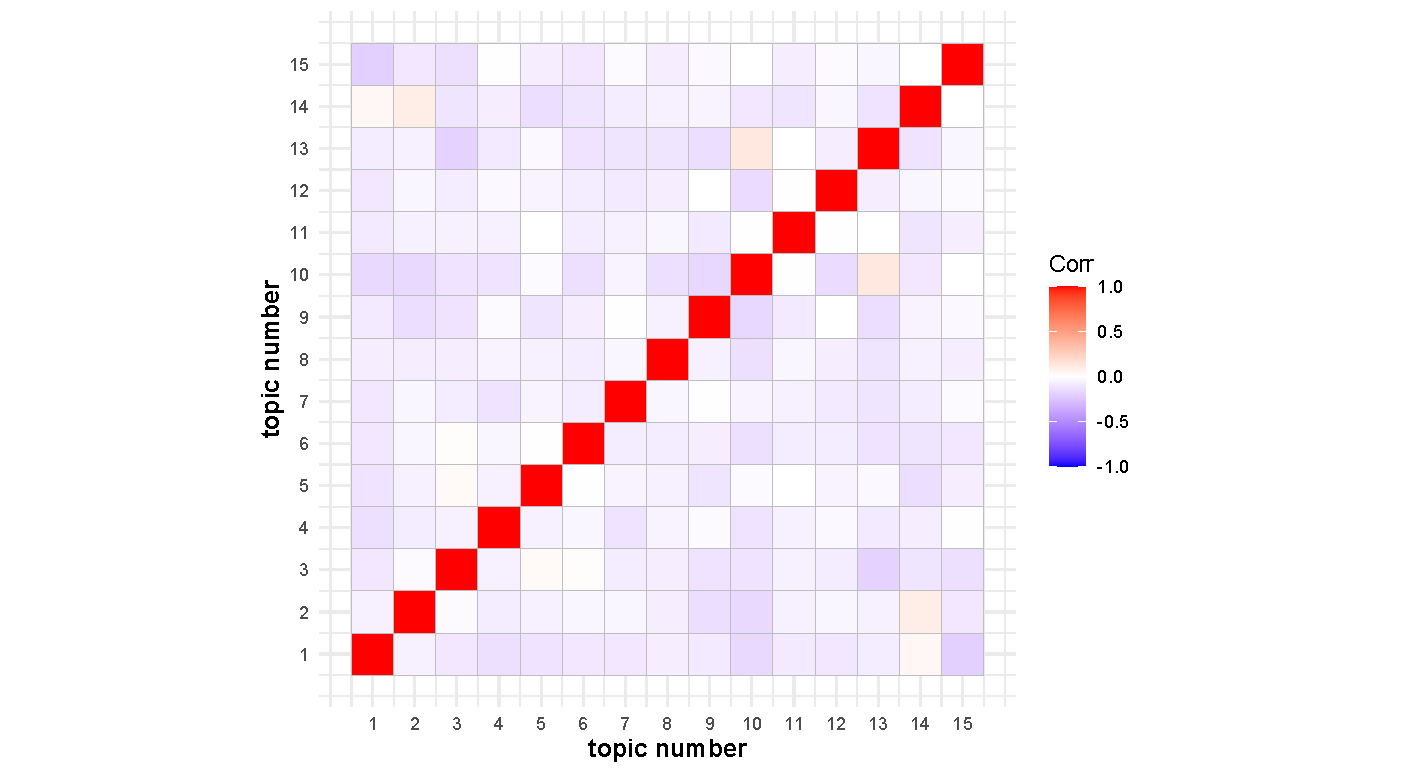
\includegraphics[width=\linewidth]{../plots/4_3/topic_correlations.pdf}
  \end{subfigure}
  \begin{subfigure}[b]{0.4\linewidth}
    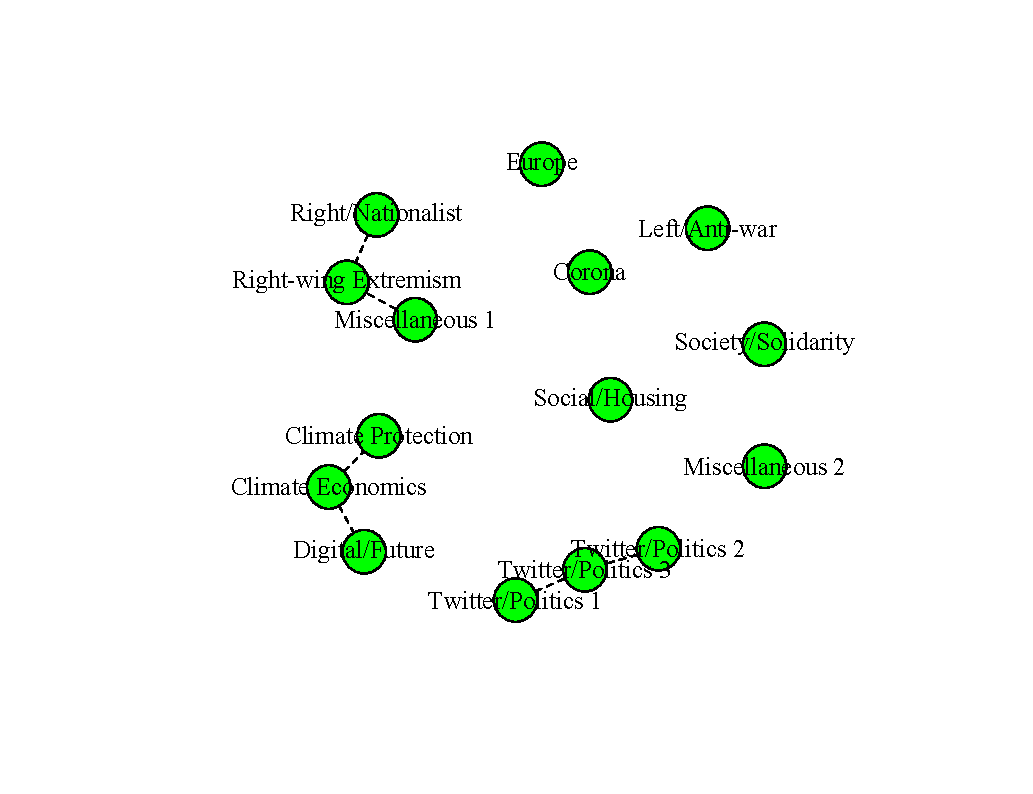
\includegraphics[width=\linewidth]{../plots/4_3/topic_correlations_map.pdf}
  \end{subfigure}
  \caption{Global topic correlations as matrix (left) and graph (left).}
  \label{fig:topic_correlations}
\end{figure}